\documentclass[fleqn,letterpaper,12pt,printwatermark=false]{memoir}
% memoir commands to define the text block geometry
\setulmarginsandblock{0.5in}{*}{*}
\setlrmarginsandblock{0.5in}{*}{*}
% put "extra" vertical space at the bottom of a page
\raggedbottom 

\usepackage{amsmath}
\usepackage{xparse} % for NewDocumentCommand et al.
\usepackage{enumitem}
\usepackage{transparent} % for \transparent, which I use in the watermark
\usepackage[slantedGreek]{mathpazo} \usepackage{helvet} % use Palatino et al.
\usepackage{booktabs} % prettier tables

\usepackage[]{xwatermark}
\newwatermark*[
    allpages,
    color=red!30,angle=45,
    scale=4,
    xpos=-10, ypos=0
]{%
    \transparent{0.4}dhasan example%
}

\usepackage{dashundergaps} % for \gap
\dashundergapssetup{
    teacher-mode=true, % set to true to show answers 
    gap-format=underline,
    teacher-gap-format=underline,
    gap-font={\sffamily},
    gap-numbers=true,
    gap-widen=true,
    gap-extend-percent=150, % note: making this too big might create errors
    gap-number-format=\,\textsuperscript{\normalfont(\thegapnumber)},
}

\usepackage{tcolorbox}
\tcbuselibrary{skins}
\tcbuselibrary{raster}

\usepackage{pgfplots}
\pgfplotsset{compat=newest}

% ---------------------DOCUMENT------------------------------
\begin{document}

\newcommand{\myClassName}{Pre-AP Algebra 2}
\newcommand{\myUnitNumber}{1}
\newcommand{\myUnitTitle}{Introduction to Functions}
\newcommand{\myLessonNumber}{10}
\newcommand{\myLessonTitle}{Sketching Inverses}


\copypagestyle{myPagestyle}{empty}


\newcommand{\myFooterSize}{\footnotesize}
\makeoddfoot{myPagestyle}{{}}{\myFooterSize{\thepage{}~of~\pageref*{xwmlastpage}}}{\myFooterSize\thetitle}
\makeevenfoot{myPagestyle}{{}}{\myFooterSize{\thepage{}~of~\pageref*{xwmlastpage}}}{\myFooterSize\thetitle}

%
% A command to change the appearance of the cognitive verb 
% in the objectives.
%
\newcommand{\myCognitiveVerb}[1]{\textcolor{blue}{\textbf{#1}}}

%
% Terminology explanation:
%
% "unit" refers to the Algebra 2 unit being taught.
% "section" refers to the section within the unit being taught.
% "heading" refers to the headings in this document (Objectives, Example, ...)
%
\NewDocumentCommand{\myUnitSectionNumberFont}{}{\sffamily\bfseries\HUGE}
\NewDocumentCommand{\myUnitNameFont}{}{\sffamily\large}
\NewDocumentCommand{\mySectionNameFont}{}{\sffamily\bfseries\huge}
\NewDocumentCommand{\myHeadingFont}{}{\sffamily\bfseries\Large}


%
% #1 is the fill-in text
%
\NewDocumentCommand{\myFillInBlank}{m}{%
    \,%
    \gap[u]{#1}%
    \,%
}


% Definition for the LESSON HEADER + OBJECTIVES
%
% #1 : optional unit name
% #2 : optional unit/section number
% #3 : mandatory title
%
\NewDocumentEnvironment{myNotesHeader}{oom}{
    \title{#3}
    \begin{flushleft}
        \IfValueT{#2}{{\myUnitSectionNumberFont#2}}
        \hfill\;\;
        \begin{minipage}[b]{0.75\textwidth}
            \begin{flushright}
                \IfValueT{#1}{
                    {\myUnitNameFont#1}\\ \vspace{0.75em}
                }
                {\mySectionNameFont#3}
            \end{flushright}
        \end{minipage}
        \hrule
    \end{flushleft}
    \noindent{\myHeadingFont Objectives:}
    \begin{enumerate}[label=\arabic*)]
}{
    \end{enumerate}
}


% Definitions related to the VOCABULARY TABLE
%
\newenvironment{myVocabulary}{
    {\noindent{\myHeadingFont Vocabulary:}}\vspace{1em}

    \begin{tabular}{ll}
        \toprule
            \emph{word} & \emph{meaning} \\ 
        \midrule
}{
    \bottomrule
    \end{tabular}
    \vspace{1em}
}

\newcommand{\myVocabularyWord}[2]{%
{\textcolor{blue}{\textbf{#1}}} & #2 \\
}


% Definitions related to an INTRODUCTION
%
\newenvironment{myIntroduction}{
    {\noindent{\myHeadingFont Introduction:}}\vspace{1em}

    \setlength{\leftskip}{3cm}
}{
    \setlength{\leftskip}{0pt}
}


% Definition related to KEY CONCEPTS
%
% #1 : the key concept (which appears as a tcolorbox title)
%
\NewDocumentEnvironment{myKeyConcepts}{ O{Key Concepts:} }{
    \begin{tcolorbox}[
        title=#1, fonttitle=\myHeadingFont,
        coltitle=black, 
        colbacktitle=black!25!yellow, 
        colframe=black!50!yellow,
        colback=white!70!yellow,
        boxrule=2pt, 
        ]
}{
    \end{tcolorbox}
}


% Definition related to EXAMPLES
%
% #1 Optional example number 
% #2 A statement of the example problem.
% #3 How much empty vertical space to leave for the example box.
%
\NewDocumentCommand{\myExample}{omm}{%
    \begin{tcolorbox}[
        enhanced,
        sharp corners, 
        colback=white,
        boxrule=0pt,
        borderline={0.5pt}{0pt}{black,dashed},
        ]
        {\myHeadingFont Example\IfValueT{#1}{{ #1}}:}
        #2
        \tcblower
        \vspace{#3}
    \end{tcolorbox}
}

% Definitions related to PROBLEMS

% A counter to number the problems in the guided notes.
\newcounter{MyProblemCounter}
\setcounter{MyProblemCounter}{1}
\newcommand{\useMyProblemCounter}{\theMyProblemCounter\stepcounter{MyProblemCounter}}

% an environment for two adjacent problems
%
% #1 : directions for all the problems
% #2 : vertical height of the problem boxes
% #3 : details for problem 1
% #4 : details for problem 2
%
\newenvironment{myProblems2}[4]{%
    \noindent
    {\myHeadingFont Practice:}\hspace{0.5em}#1\nopagebreak%
    \begin{tcbraster}[%
        raster equal height,%
        raster columns=2,%
        raster column skip=0.5mm,%
        raster row skip=0.5mm,%
        raster every box/.style={%
            enhanced,%
            sharp corners,%
            colback=white,%
            coltitle=black, colbacktitle=black!10!white,%
            boxrule=0pt, borderline={0.5pt}{0pt}{black},%
            title={\texttt\useMyProblemCounter},%
            },%
        ]%
        \begin{tcolorbox}[attach boxed title to top left]
            #3
            \tcblower\vspace{#2}
        \end{tcolorbox}
        \begin{tcolorbox}[attach boxed title to top right]
            #4
            \tcblower
        \end{tcolorbox}%
}{%
    \end{tcbraster}
}

% an environment for 4 adjacent problems
%
% #1 : directions for all the problems
% #2 : vertical height of the problem boxes
% #3 : details for problem 1
% #4 : details for problem 2
% #5 : details for problem 3
% #6 : details for problem 4
%
\newenvironment{myProblems4}[6]{%
    \noindent
    \textbf{\myHeadingFont Practice:}\hspace{0.5em}#1\nopagebreak%
    \begin{tcbraster}[%
        raster equal height,%
        raster columns=2,%
        raster column skip=0.5mm,%
        raster row skip=0.5mm,%
        raster every box/.style={%
            enhanced,%
            sharp corners,%
            colback=white,%
            coltitle=black, colbacktitle=black!10!white,%
            boxrule=0pt, borderline={0.5pt}{0pt}{black},%
            title={\texttt\useMyProblemCounter},%
            },%
        ]%
        \begin{tcolorbox}[attach boxed title to top left]
            #3
            \tcblower\vspace{#2}
        \end{tcolorbox}
        \begin{tcolorbox}[attach boxed title to top right]
            #4
            \tcblower
        \end{tcolorbox}%
        \begin{tcolorbox}[attach boxed title to bottom left]
            #5
            \tcblower
        \end{tcolorbox}%
        \begin{tcolorbox}[attach boxed title to bottom right]
            #6
            \tcblower
        \end{tcolorbox}%
}{%
    \end{tcbraster}
}
\pagestyle{myPagestyle}

\checkandfixthelayout
\setlist{labelindent=\parindent,leftmargin=*,itemsep=0.025em,label=$\circ$}

% ---------------------LESSON------------------------------
\begin{myNotesHeader}
    \item \myCognitiveVerb{sketch} the graph of the inverse of a function
\end{myNotesHeader}

\begin{myVocabulary}
    \myVocabularyWord{sketch}
        {
            draw something quickly without being perfect
        }
    \myVocabularyWord{inverse functions}
        {
            two functions that ``undo'' each other
        }
\end{myVocabulary}

% ---------------------LESSON------------------------------
\begin{myLesson}
    In lesson 1.9 you learned how to find the inverse $f^{-1}$ 
    for a function $f$.
    It was a lot of ``algebra''.
    The key part of those \emph{algebraic} steps was {\bfseries swapping} 
    the $x$ and $y$ variables. 
    What does that mean \emph{geometrically} (visually)?
    In this lesson, we will graph some inverses to find out.

    You should learn two things:

    \begin{myLessonBox}
        Graphing the inverse of $f$ is really just a matter 
        of figuring out what $f^{-1}$ first. 
        Then you just sketch it.
    \end{myLessonBox}

    \begin{myLessonBox}
        If you visually compare the graph of a function
        to the graph of its inverse,
        you will see that they are \emph{mirror images} (reflections)
        across the diagonal line, $y=x$.
    \end{myLessonBox}
\end{myLesson}

% ---------------------CONCEPT 1------------------------------
\begin{myKeyConcepts}[To sketch the inverse of $f(x)$\dots]
    Follow these steps:
    \setlist{labelindent=\parindent,itemsep=0.4em}
    \begin{enumerate}
        \item Find the inverse function $f^{-1}(x)$ using what you learned in Lesson 1.9.
        \item Sketch the graph of that inverse function 
        (by hand if you know how to graph it or using a graphing calculator or Desmos to help you if you don't).
    \end{enumerate}
\end{myKeyConcepts}

\myExample[1]{
    Sketch the graph of the inverse of
    \( f(x) = 3x \)
}{2.75in}

\myExample[2]{
    Sketch the graph of the inverse of
    \( v(t) = 2t-7 \)
}{2.75in}

\myExample[3]{
    Sketch the graph of the inverse of
    \( f(x) = \frac{2}{5}x- \frac{1}{5} \)
}{2.75in}

% ---------------------CONCEPT 2------------------------------
\begin{myKeyConcepts}[To see the visual relationship between a function and its inverse\dots]
    Follow these steps:
    \setlist{labelindent=\parindent,itemsep=0.4em}
    \begin{enumerate}
        \item Sketch the graph of the original function $y = f(x)$.
        \item Sketch the graph of the inverse function $y = f^{-1}(x)$.
        \item Lightly sketch the graph of the diagonal line, $y=x$ (or draw it as a dotted line).
        \item Notice that the graph of the inverse function 
        is the mirror image (reflection) of the original function 
        across that diagonal line.
    \end{enumerate}
\end{myKeyConcepts}

\begin{myExampleForTikzGraphs}*[4]{
    Let's consider the function 
    \( f(x) = x^5 \).
    It turns out (we will learn this later in the year)
    that the inverse of this function its
    \( f^{-1}(x) = \sqrt[5](x) \).
}
    We could (but you don't need to) use a graphing calculator or Desmos to graph $f$ and $f^{-1}$:

    \begin{center}
    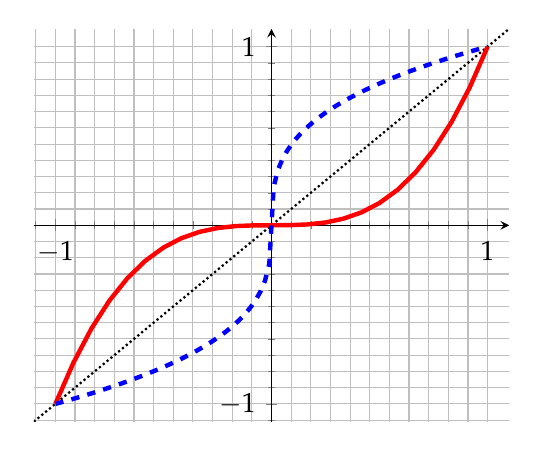
\begin{tikzpicture}
    \begin{axis}[
        width=3in,
        grid=both,
        axis x line = middle,axis y line = middle,
        % axis equal image,
        xtick distance = 1, ytick distance = 1,
        minor tick num=10,
        ]
        \addplot[no marks,densely dotted,thick,domain=-1.1:1.1]{x};
        \addplot[no marks,solid,red,ultra thick,domain=-1:1]{x^3};
        % cube root, see: https://tex.stackexchange.com/questions/69411/pgfplots-cant-plot-some-usual-mathematical-functions
        \addplot[no marks,solid,blue,dashed,ultra thick,domain=-1:1,samples=100]{x/abs(x)*abs(x)^(1/3)};
    \end{axis}
    \end{tikzpicture}
    \end{center}
    
    \noindent Notice how the two graphs are {\bfseries mirror image reflections} of each other 
    across the diagonal line.
\end{myExampleForTikzGraphs}

% \begin{myProblems2}%
%     {Factor the following monomials into prime factors.}%
%     {2in}%
%     %
%     {\( 32x^2 \)}
%     {\( 8 x^3y^2z \)}
% \end{myProblems2}
  


\end{document}